\documentclass[12pt,a4paper]{article}
\usepackage[utf8]{inputenc}
\usepackage[T2A]{fontenc}
\usepackage[russian]{babel}
\usepackage{amsmath,amsfonts,amssymb}
\usepackage{graphicx}
\usepackage{geometry}
\usepackage{multirow}
\usepackage{float}
\usepackage{caption}
\usepackage{enumitem}
\geometry{top=2cm,bottom=2cm,left=2.5cm,right=1.5cm}

\newcommand{\deriv}[2]{\frac{\partial #1}{\partial #2}}
\newcommand{\derivt}[1]{\frac{\partial #1}{\partial t}}
\newcommand{\aver}[1]{\langle #1 \rangle}
\renewcommand{\labelitemi}{$\bullet$}

\begin{document}

\begin{titlepage}
    \begin{center}
        \textbf{Московский физико-технический институт (национальный исследовательский университет)} \\
        \textbf{Физтех-школа аэрокосмических технологий (ФАКТ)} \\
        \vspace{3cm}
        \Large{Лабораторная работа №8} \\
        \Huge{МЕТОДЫ ГЕНЕРАЦИИ И РЕГИСТРАЦИИ УДАРНЫХ ВОЛН} \\
        \vspace{2cm}
        \large{Работу выполнили:} \\
        \large{Позывай Павел Вячеславович} \\
        \large{Танов Константин Леонидович} \\
        \large{Реджепдурдыев Бердигылыч} \\
        \large{Цветкова Амелия Антоновна} \\
        \large{Сергеев Константин Андреевич} \\
        \vfill
        \large{Группа Б03-305} \\
        \large{Долгопрудный, 2026}
    \end{center}
\end{titlepage}

\tableofcontents
\newpage

\section{Цель работы}
Целью лабораторной работы является ознакомление с ударными трубами как инструментом для получения ударных волн в лабораторных условиях, освоение методов регистрации и измерения интенсивности ударных волн, а также экспериментальное построение зависимости интенсивности ударной волны $p_2/p_1$ от начального перепада давлений на диафрагме $p_4/p_1$ для ударной трубы переменного сечения и сравнение полученных результатов с теоретической моделью.

\section{Теоретическая часть}
\subsection{Основы работы ударной трубы}
Простейшая ударная труба представляет собой длинный канал постоянного сечения, разделённый диафрагмой на две части: камеру высокого давления (КВД) с давлением $p_4$ и камеру низкого давления (КНД) с давлением $p_1$ ($p_4 > p_1$). При мгновенном удалении диафрагмы возникает сложная волновая картина: по газу низкого давления распространяется ударная волна, а по газу высокого давления — центрированная волна разрежения. Области за ударной волной (область~2) и за волной разрежения (область~3) разделены контактной поверхностью (рис. \ref{fig:812}), на которой давление и скорость непрерывны: $p_2 = p_3$, $u_2 = u_3$, а плотность и температура терпят разрыв.

\subsection{Определение параметров газа на ударном фронте}
Для совершенного газа с постоянным показателем адиабаты $\gamma$ на стационарном прямом скачке уплотнения справедливы соотношения Рэнкина–Гюгонио. В системе координат, где невозмущённый газ покоится, скорость ударной волны $N$ и число Маха ударной волны $M_s = N/a_1$ связаны с интенсивностью:
\begin{equation}
    M_s = \sqrt{ \frac{\gamma-1}{2\gamma} + \frac{\gamma+1}{2\gamma}\,\frac{p_2}{p_1} } \quad \text{или} \quad
    \frac{p_2}{p_1} = \frac{2\gamma}{\gamma+1} M_s^2 - \frac{\gamma-1}{\gamma+1}.
    \label{eq:Ms}
\end{equation}
Скорость газа за фронтом $u_2$ определяется выражением:
\begin{equation}
    \frac{u_2}{a_1} = \frac{2}{\gamma+1}\left(M_s - \frac{1}{M_s}\right).
    \label{eq:u2a1}
\end{equation}
Обратная зависимость $p_2/p_1$ от $u_2/a_1$ может быть получена итерационно (см.~раздел~4).

\subsection{Теоретическая зависимость интенсивности от начальных давлений в КВД и КНД}
В установке УТ-2 сечение КВД ($F_4$) меньше сечения канала ($F_1$), они соединены расширяющимся соплом. Это делается для ослабления интенсивности ударной волны и улучшения её формирования. Расчёт такой конфигурации усложняется: в зависимости от перепада давлений на входе в сопло может устанавливаться либо дозвуковой режим течения, либо звуковой с последующим возникновением прямого скачка уплотнения внутри сопла.

Рассматривался случай, когда и КВД, и канал наполнены воздухом: \(\gamma = 1.4\). Волна разрежения, образующаяся при разрыве диафрагмы, представляет собой центрированную волну, в которой каждая точка движется с постоянной скоростью \(C = a - u\), где \(a\) – местная скорость звука, \(u\) – местная скорость частиц газа. «Голова» волны движется в сторону торца КВД со скоростью, равной скорости звука \(a_4\) в невозмущенной среде. Замыкающая волну разрежения характеристика определяется уравнением:

\begin{equation}\label{eq:87}
\frac{x}{t} = c_5 = a_4 - \frac{\gamma + 1}{2} u_5.
\end{equation}

Рассмотрим случай, когда течение дозвуковое. При этом на входе сопла устанавливается дозвуковое
течение, параметры которого остаются постоянными во времени с момента разрыва
диафрагмы до прихода отраженной от торца КВД волны разрежения и определяются
формулами: 

\begin{gather}
a_5 = a_4 - \frac{\gamma-1}{2} u_5, \label{eq:a5}\\
M_5 = \frac{2}{\gamma-1}\left(\frac{a_4}{a_5}-1\right), \label{eq:M5}\\
\frac{p_5}{p_4} = \left(\frac{a_5}{a_4}\right)^{\frac{2\gamma}{\gamma-1}}. \label{eq:p5p4}
\end{gather}

Естественно предположить, что в этом случае устанавливается дозвуковое течение, для которого справедливы соотношения:

\[
q(M) = \frac{F_*}{F} = M\left[\frac{2}{\gamma+1}\left(1+\frac{\gamma-1}{2}M^2\right)\right]^{-\frac{\gamma+1}{2(\gamma-1)}}.
\]

\[
\pi(M) = \dfrac{p}{p_0} = \left(1+\dfrac{\gamma-1}{2}M^2\right)^{-\frac{\gamma}{\gamma-1}}
\]

\[
\tau(M) = \dfrac{T}{T_0} = \left(1+\dfrac{\gamma-1}{2}M^2\right)^{-1}
\]

Здесь \(a,\;p,\;M\) – параметры течения в сечении сопла с площадью \(F\), \(F_*\) – площадь критического сечения, \(q(M)\) – приведенный расход, параметры торможения. Этому случаю соответствует модель течения, представленная на рис. 1.

Индексами 1 и 4 отмечены параметры газа в невозмущенных областях соответственно в канале и КВД, 2 – в области между ударным фронтом и контактной поверхностью (т.е. в «пробке»), 3 – между выходом сопла и контактной поверхностью, 5 – между хвостом волны разрежения и входом в сопло.

\begin{figure}[h]
\centering
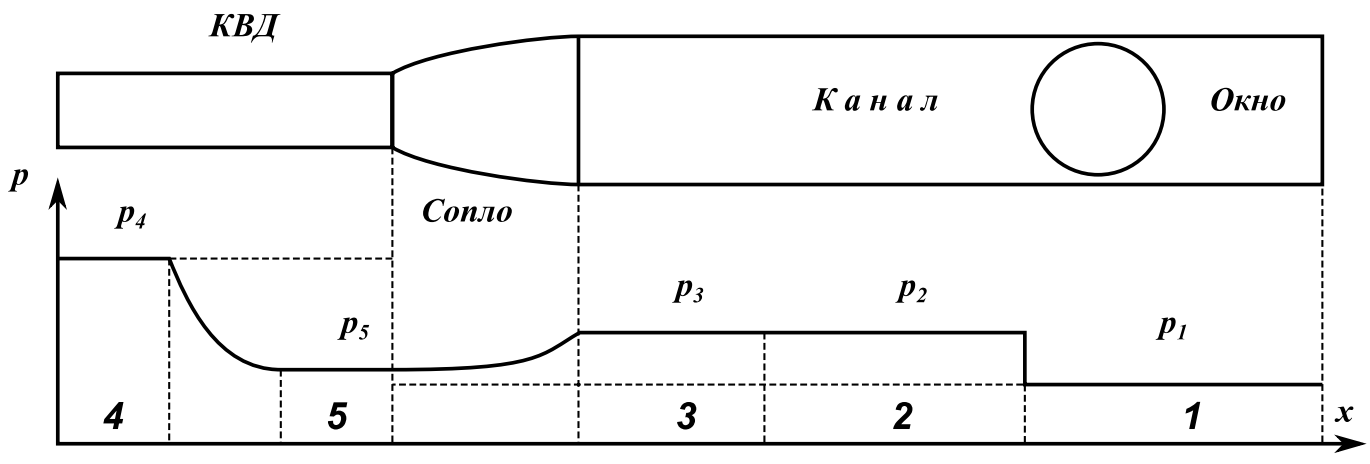
\includegraphics[width=0.9\textwidth]{Screenshot from 2026-02-17 18-05-40.png}
\caption{Модель течения при дозвуковой скорости потока на входе в сопло.}
\label{fig:812}
\end{figure}

На участке канала между выходным сечением сопла и контактной поверхностью
параметры потока неизменны. На контактной поверхности давление и скорость
неразрывны: 

\[
u_3 = u_2,\qquad p_3 = p_2.
\]

Скорости потока \(u_2\) за ударной волной соответствует определенная интенсивность ударной волны:

\begin{equation}\label{eq:83}
\frac{u_2}{a_1} = \left(\frac{p_2}{p_1}-1\right)\left[\frac{\gamma(\gamma-1)}{2}\left(1+\frac{\gamma+1}{\gamma-1}\,\frac{p_2}{p_1}\right)\right]^{-\frac{1}{2}}.
\end{equation}

Такая модель течения реализуется при \(c_5 > 0\), т.е. в пределах

\[
1 > p_5/p_4 > 0.279.
\]

Расчет зависимости интенсивности ударной волны от начального перепада давлений на диафрагме \(p_2/p_1 = f(p_4/p_1)\) для этого случая проводится по следующей схеме:
\begin{enumerate}
    \item Вводим параметр \(t = p_5/p_4 \in (0.279; 1)\). 
    \item По формуле (6) находим \(a_5/a_4\).
    \item По формуле (5) находим \(M_5\).
    \item  Так как $\frac{q(M_3)}{q(M_5)} = \frac{F_5}{F_3} = \frac{F_4}{F_1}$, то можно найти q(M3) => M3.
    \item Так как $\frac{p_3}{p_5} = \frac{\pi(M_3)}{\pi(M_5)}$, то можно найти $\frac{p_3}{p_5}$.
    \item Верно следующее: $\frac{p_2}{p_1} = \frac{p_3}{p_1} = \frac{p_4}{p_1} \frac{p_3}{p_5} \frac{p_5}{p_4}$. Значит можно найти $\frac{p_2}{p_1} = \frac{p_4}{p_1} \omega(t)$.
    \item Так как $\frac{a_3}{a_5} = \sqrt{\frac{\tau(M_3)}{\tau(M_5)}}$, то можно найти $\frac{a_3}{a_5}$.
    \item Так как в невозмущенном потоке T = const, $a = \sqrt\frac{\gamma R T}{\mu}$, то $\frac{a_4}{a_1} = 1$
    \item Верно следующее $\frac{u_2}{u_1} = \frac{u_3}{p_1} = M_3 * \frac{a_3}{a_1} = M_3 \frac{a_4}{a_1} \frac{a_3}{a_5} \frac{a_5}{a_4} = g(\frac{p_2}{p_1})$, где g - это зависимость (7). Значит можно найти $\frac{p_2}{p_1} = g^{-1}(h(t))$.
\end{enumerate}

Таким образом получена параметрическая зависимость $\frac{p_2}{p_1}(t)$ и $\frac{p_4}{p_1}(t)$.

При интенсивности волны разрежения, соответствующей \(C_5 = a_5 - u_5 = 0\), на входе сопла устанавливается критический режим течения.

\[
\begin{aligned}
u_5 &= \frac{2}{\gamma+1}\,a_4,\\[2mm]
a_5 &= a_4\left(1-\frac{\gamma-1}{2}\cdot\frac{2}{\gamma+1}\right)=a_4\frac{2}{\gamma+1},\\[2mm]
a_5 &= u_5,\qquad M_5 = 1,\qquad F_4 = F,\\[2mm]
\frac{p_5}{p_4} &= \left(\frac{2}{\gamma+1}\right)^{\frac{2\gamma}{\gamma-1}} = 0.279,\\[2mm]
\end{aligned}
\]

При дальнейшем повышении отношения давлений на диафрагме \(p_4/p_1\) в сопле развивается сверхзвуковое течение, но в некотором сечении \(F_s\) устанавливается скачок соответствующей интенсивности. Соотношения на ПСУ:

\begin{align}
M_2^2 &= \frac{1 + \frac{\gamma - 1}{2} M_1^2}{\gamma M_1^2 - \frac{\gamma - 1}{2}} \\
\frac{P_2}{P_1} &= \frac{2\gamma}{\gamma + 1} M_1^2 - \frac{\gamma - 1}{\gamma + 1} \\
\frac{T_2}{T_1} &= \frac{(2\gamma M_1^2 - \gamma + 1)((\gamma - 1) M_1^2 + 2)}{(\gamma + 1)^2 M_1^2}
\end{align}

Здесь индексы 1–5 имеют тот же смысл, что и на рис. 8.12; индексом 6 отмечено состояние газа перед скачком, индексом 7 – сразу за скачком; параметрам газа в выходном сечении сопла соответствует индекс 3.

Расчет зависимости интенсивности ударной волны от начального перепада давлений на диафрагме \(p_2/p_1 = f(p_4/p_1)\) для этого случая проводится по следующей схеме:
\begin{enumerate}
    \item Вводим параметр \(t = F_s \in [1; 5]\). 
    \item  Так как $\frac{q(M_5)}{q(M_6)} = \frac{F_6}{F_5} = \frac{F_4}{F_s}$, то можно найти q($M_6$) => $M_6$.
    \item Из формулы (8) можно найти $M_7$.
    \item  Так как $\frac{q(M_3)}{q(M_7)} = \frac{F_7}{F_3} = \frac{F_s}{F_1}$, то можно найти q($M_3$) => $M_3$.
    \item Так как $\frac{p_3}{p_7} = \frac{\pi(M_3)}{\pi(M_7)}$, то можно найти $\frac{p_3}{p_7}$.
    \item По формуле (9) можно найти $\frac{p_7}{p_6}$.
    \item Так как $\frac{p_6}{p_5} = \frac{\pi(M_6)}{\pi(M_5)}$, то можно найти $\frac{p_6}{p_5}$.
    \item Верно следующее: $\frac{p_2}{p_1} = \frac{p_3}{p_1} = \frac{p_4}{p_1} \frac{p_3}{p_7} \frac{p_7}{p_6} \frac{p_6}{p_5} \frac{p_5}{p_4}$. Значит можно найти $\frac{p_2}{p_1} = \frac{p_4}{p_1} \omega(t)$.
    \item Так как $\frac{a_3}{a_7} = \sqrt{\frac{\tau(M_3)}{\tau(M_7)}}$, то можно найти $\frac{a_3}{a_7}$.
    \item Так как в невозмущенном потоке $a = \sqrt\frac{\gamma R T}{\mu}$, то $\frac{a_4}{a_1} = 1$
    \item По формуле (10) можно найти $\frac{a_7}{a_6}$.
    \item Так как $\frac{a_6}{a_5} = \sqrt{\frac{\tau(M_5)}{\tau(M_5)}}$, то можно найти $\frac{a_6}{a_5}$.
    \item Верно следующее $\frac{u_2}{u_1} = \frac{u_3}{p_1} = M_3 * \frac{a_3}{a_1} = M_3 \frac{a_4}{a_1} \frac{a_3}{a_7} \frac{a_7}{a_6} \frac{a_6}{a_5} \frac{a_5}{a_4} = g(\frac{p_2}{p_1})$, где g - это зависимость (7). Значит можно найти $\frac{p_2}{p_1} = g^{-1}(h(t))$.
\end{enumerate}

Таким образом получена параметрическая зависимость $\frac{p_2}{p_1}(t)$ и $\frac{p_4}{p_1}(t)$.

\section{Экспериментальная установка и методика измерений}
\subsection{Описание ударной трубы УТ-2}
Установка УТ-2 представляет собой одноступенчатую ударную трубу переменного сечения. КВД цилиндрическая (длина 0.5~м, максимальное давление 30~атм), КНД прямоугольного сечения 45×90~мм (длина около 2.6~м до измерительного отсека, давление до 10~атм). Камеры разделены диафрагмой, которая разрушается поворотным механизмом с иглой. Измерительный отсек снабжён оптическими окнами для лазерных измерений и пьезодатчиком давления.

\subsection{Система лазерного измерения скорости ударной волны}
Скорость фронта ударной волны определяется по времени прохождения базового расстояния $\ell = 5$~см между двумя параллельными лазерными лучами. Лучи формируются полупроводниковыми лазерами и направляются через измерительную секцию на фотодиоды. При прохождении ударного фронта показатель преломления газа скачкообразно меняется (закон Гладстона–Дейла), луч отклоняется, что изменяет освещённость фотодиодов. На осциллограмме возникают два характерных пика. Измеряя задержку $\Delta t$ между ними, находят скорость фронта:
\[
N = \frac{\ell}{\Delta t},\quad M_s = \frac{N}{a_1},
\]
где $a_1 = \sqrt{\gamma R T_1/\mu}$ — скорость звука в невозмущённом газе.

\subsection{Измерение интенсивности ударной волны пьезодатчиком}
В стенке измерительного отсека установлен пьезоэлектрический датчик давления PCB 113B21 (чувствительность $k = 3.6$~мВ/кПа). При прохождении ударной волны кристалл деформируется, вырабатываемый заряд преобразуется формирователем в напряжение $U$, пропорциональное скачку давления $\Delta p = p_2-p_1$:
\[
p_2-p_1 = \frac{\Delta U}{k}.
\]
Зная начальное давление $p_1$ (измеряется мановакуумметром), находим $p_2/p_1 = 1 + \Delta p/p_1$.

\section{Результаты и обсуждение}
В эксперименте были получены данные для семи различных начальных давлений $p_1$ и $p_4$. Атмосферное давление в день эксперимента составляло $752 ~\text{мм. рт. ст.}$, температура $T=297$~К. Скорость звука $a_1 = \sqrt{\gamma R T/\mu} \approx 345$~м/с.

На рис.~\ref{fig:graph} представлено сравнение экспериментальных точек с теоретической кривой, рассчитанной для $F_1/F_4=5$, $\gamma=1.4$, $a_1=a_4$. Для нахождения отклонения использована полуширина пика напряжения на осциллографе на высоте $1/\sqrt{2}$ (1.17 мкс).

\begin{figure}[H]
\centering
\includegraphics[width=1.1\textwidth]{graph_err.png}
\caption{Зависимость интенсивности ударной волны $p_2/p_1$ от начального перепада давлений $p_4/p_1$. Сплошная линия — теория (дозвуковой режим), штриховая — теория со скачком, точки — эксперимент.}
\label{fig:graph}
\end{figure}

Анализ полученных данных позволяет сделать следующие наблюдения:
\begin{itemize}
    \item Экспериментальные точки систематически лежат ниже теоретической кривой. Это можно объяснить вязкостью - диссипацией энергии ударной волны.
    \item Значения $p_2/p_1$, полученные "лазерным" методом (по скорости фронта ударной волны), оказались существенно ниже значений, полученных прямым измерением давления пьезодатчиком.
\end{itemize}

\newpage
\section{Выводы}
В ходе выполнения лабораторной работы:
\begin{enumerate}
    \item Экспериментально исследована ударная труба переменного сечения УТ-2; освоены методы регистрации ударных волн с помощью лазерной системы и пьезодатчика давления.
    \item Построена теоретическая зависимость интенсивности ударной волны $p_2/p_1$ от начального перепада давлений $p_4/p_1$.
    \item Проведено сравнение экспериментальных данных с теоретической моделью.
    \item Установлено, что экспериментальные точки лежат ниже теоретической кривой, что объясняется диссипацией. Также влияние может оказывать утечка воздуха из КВД и в КНД.
    \item Обнаружено расхождение между значениями $p_2/p_1$, полученными лазерным методом и прямым измерением давления. Погрешность измерения $p_2/p_1$ лазером сильно зависит от точности измерения момента прохождения фронта. Большое влияние оказывает "неидеальность" фронта: фронт может быть не плоским, а если плоский, может проходить участок измерения под углом. Даже отклонения 3-5 $\%$ при измерении времени приводят к погрешности определения интенсивности порядка 30\%.
\end{enumerate}

\end{document}
